%This is my super simple Real Analysis Homework template

\documentclass{article}
\usepackage[utf8]{inputenc}
\usepackage[english]{babel}
\usepackage[]{amsthm} %lets us use \begin{proof}
\usepackage[]{amssymb} %gives us the character \varnothing
\usepackage[]{amsmath}

\title{Homework 3}
\author{Chu Hai Nam MSSV: 2370189 \\
        Diep Le Vy MSSV: 2370200 \\
        Huynh Huy Vu MSSV: 2370199 \\
        Nguyen Truong An MSSV: 2370388\\
        Khuat Hoang tri MSSV: 2370127}
\date\today
%This information doesn't actually show up on your document unless you use the maketitle command below

\begin{document}
\maketitle %This command prints the title based on information entered above

\section*{Theorem 3.12}
    The vertex cover problem is NP-complete.

\begin{proof}
    We will proof this problem is NP-complete by proofing this is both in NP and NP-hard.
    \begin{itemize}
        \item \textbf{NP:} \\
        We will proof that the vertex cover problem is in NP by showing that the certificate is the vertex cover.\\
        Given the graph $G = (V,E)$ and k is interger.\\
        \textbf{Certificate:} A set of vertices, the vertex cover $V'\subseteq V$\\
        \textbf{Verifier:} Check if the set $V'$ is a vertex cover of size k in $G$.\\
        If the set $V'$ is a vertex cover of size k in $G$, then the certificate is accepted.\\
        If the certificate is accepted, then the set $V'$ is a vertex cover of size k in $G$.\\
        \textbf{Proof:} The verifier can check if the set $V'$ is a vertex cover of size k in $G$ by checking if for every edge $(u,v) \in E$, either $u \in V'$ or $v \in V'$.\\
        The running time is polynominal time thus the vertex cover problem is in NP.

        \item \textbf{NP-hard:} \\
        We will proof that the vertex cover problem is NP-hard by reducing the vertex cover problem to the clique problem.\\
        Given the graph $G = (V,E)$ and k is interger.\\
        \textbf{Reduction:} Construct a new graph $G' = (V',E')$ where $V' = V$ and $E' = \{(u,v) | (u,v) \notin E\}$.\\
        \textbf{Claim:} $G$ has a vertex cover of size k if and only if $G'$ has a clique of size $|V| - k$.\\
        \textbf{Proof:} \\
        \begin{itemize}
            \item If $G$ has a vertex cover of size k, then $G'$ has a clique of size $|V| - k$.\\
            Let $V'$ be the vertex cover of size k in $G$.\\
            Let $V'' = V - V'$, then $|V''| = |V| - k$.\\
            Since $V'$ is the vertex cover of size k in $G$, then for every edge $(u,v) \in E$, either $u \in V'$ or $v \in V'$.\\
            Thus, for every edge $(u,v) \notin E$, both $u \in V''$ and $v \in V''$.\\
            Therefore, $V''$ is a clique of size $|V| - k$ in $G'$.
            \item If $G'$ has a clique of size $|V| - k$, then $G$ has a vertex cover of size k.\\
            Let $V''$ be the clique of size $|V| - k$ in $G'$.\\
            Let $V' = V - V''$, then $|V'| = k$.\\
            Since $V''$ is the clique of size $|V| - k$ in $G'$, then for every edge $(u,v) \notin E$, both $u \in V''$ and $v \in V''$.\\
            Thus, for every edge $(u,v) \in E$, either $u \in V'$ or $v \in V'$.\\
            In other words, for every edge $(u,v) \in E$, at least one of $u$ and $v$ is in $V'$.\\
            $V-V'$ is a clique of size $|V| - |V'| = k$ in $G$.\\
            Therefore, $V'$ is the vertex cover of size k in $G$.
        \end{itemize}
    \end{itemize}
    
    Since the vertex cover problem is both in NP and NP-hard, the vertex cover problem is NP-complete.

\end{proof}

\section*{Theorem 3.13}
    The hamiltonian cycle problem is NP-complete.

\begin{proof}
    We will proof this problem is NP-complete by proofing this is both in NP and NP-hard.
    \begin{itemize}
        \item \textbf{NP:} \\
        We will proof that the HAM-CYCLE problem is in NP by showing that the certificate is hamiltonian cycle.\\
        Given the graph $G = (V,E)$\\
        \textbf{Certificate:} A sequence of $|V|$ vertices that makes up the hamiltonian cycle\\
        \textbf{Verifier:} Check this sequence contains each vertex in $V$ exactly once.\\
        And check the edge between pair of consecutive vertices (include first and last vertices in $V$) is exist or not.\\
        \textbf{Proof:} This certificate can be verified in polynomial time ($O(|V|) = O(1)$) so the HAM-CYCLE is NP.

        \item \textbf{NP-hard:} \\
        We will proof that the vertex cover problem is NP-hard by reducing the vertex cover problem to the clique problem.\\
        Given the graph $G = (V,E)$ and k is interger.\\
        \textbf{Reduction:} Given an undirected graph $G = (V,E)$ and an integer $k$, we construct an undirected graph $G' = (V',E')$ \\
        that has a hamiltonian cycle if and only if $G$ has a vertex cover of size $k$.\\
        $\forall$ pair vertices $u, v$. We create a widget show below
        \begin{figure}
            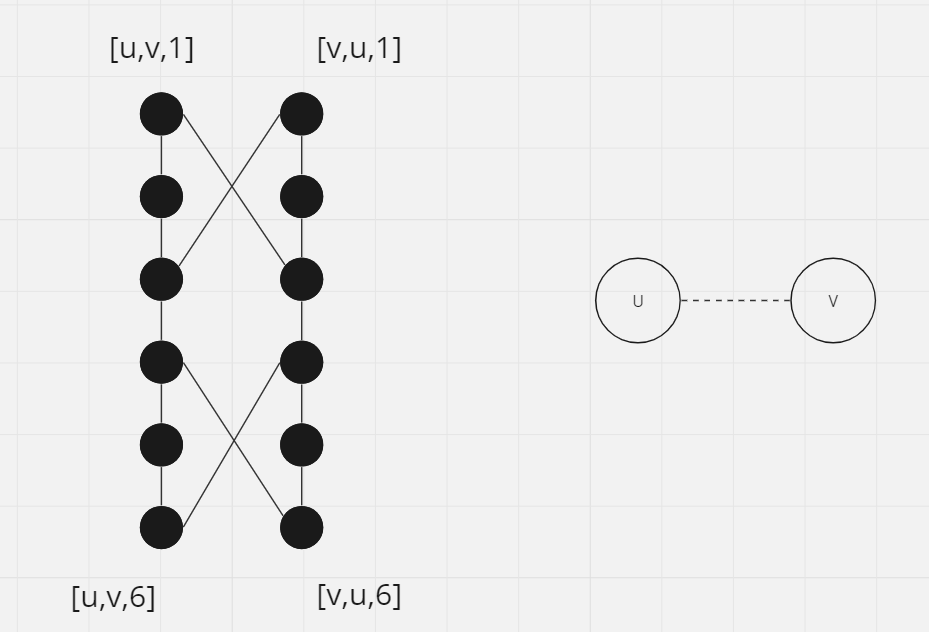
\includegraphics[width=\linewidth]{Figure_1.png}
            \caption{Widget for a pair verices u, v}
            \label{fig:1}
        \end{figure}
        With two vertices we have three case in $Figure_2$ match with $Figure_3$.
        \begin{figure}
            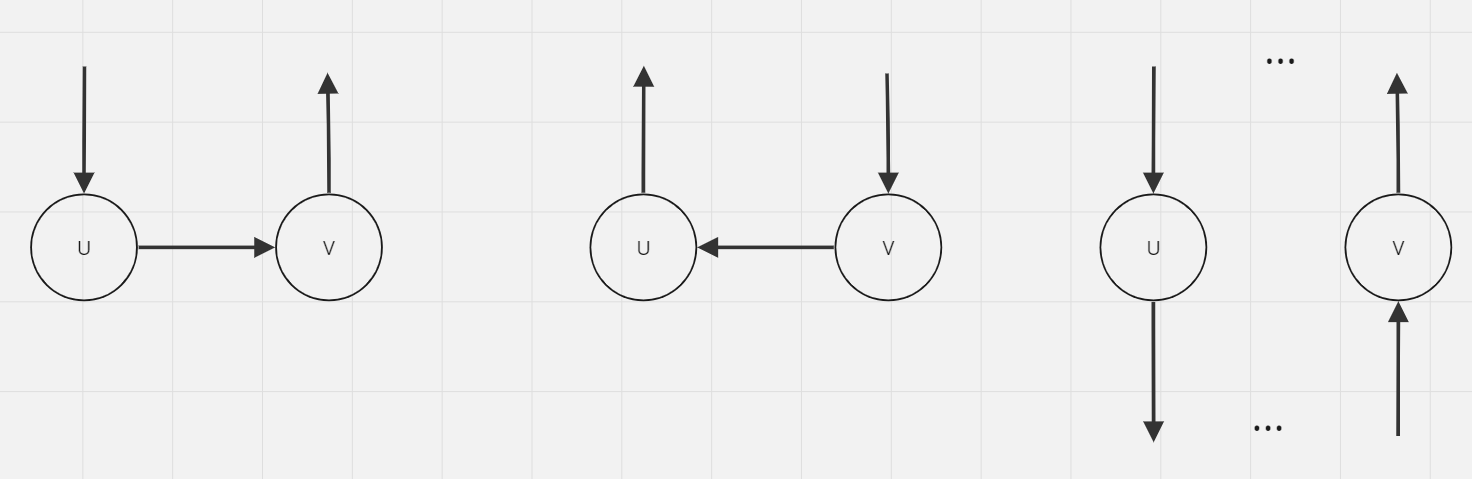
\includegraphics[width=\linewidth]{Figure_2.png}
            \caption{State of pair vertices if in HAM-CYCLE}
            \label{fig:2}
        \end{figure}
        \begin{figure}
            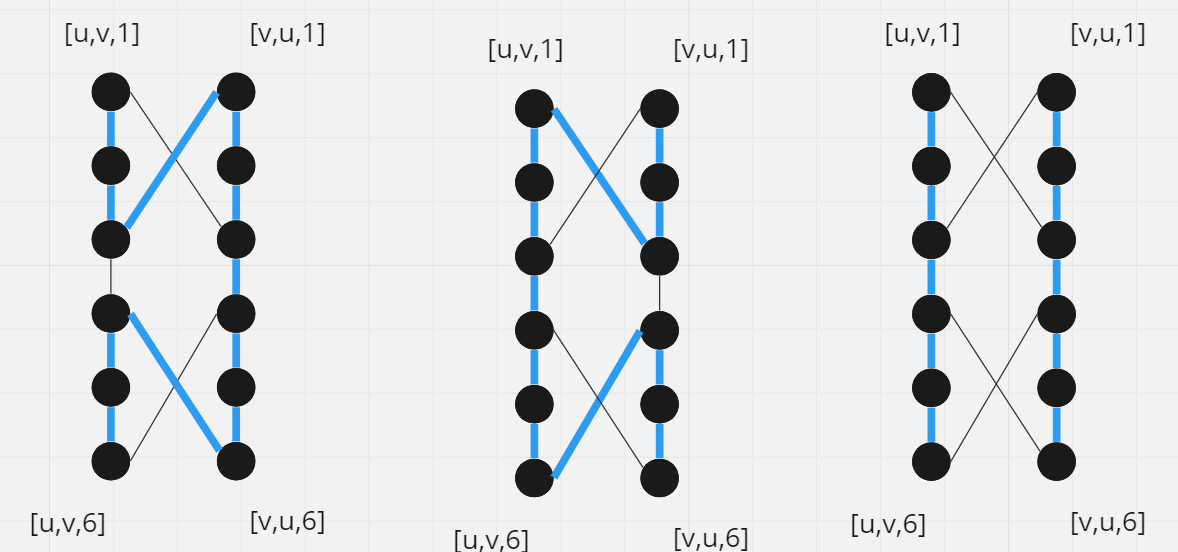
\includegraphics[width=\linewidth]{Figure_3.png}
            \caption{State of widget}
            \label{fig:3}
        \end{figure}
        Reduction construcs one widget per edge \\
        Plus k selector vertices \\
        $(u,v)$ sides of widgets connect into chains representing edges incident on each vertex $u$ \\
        Selectors are “placeholders” that can be “filled in” to represent any vertex, and so are connected to start and end of each chain \\
        \textbf{Proof:} \\
        \begin{itemize}
            \item Next we show that the size of $G^{\prime}$ is polynomial in the size of $G$, \\
            and hence it takes time polynomial in the size of $G$ to construct $G^{\prime}$. \\
            The vertices of $G^{\prime}$ are those in the gadgets, plus the selector vertices. \\
            With 12 vertices per gadget, plus $k \leq|V|$ selector vertices, $G^{\prime}$ contains a total of \\
            $$
            \begin{aligned}
            \left|V^{\prime}\right| & =12|E|+k \\
            & \leq 12|E|+|V|
            \end{aligned}
            $$
            vertices. The edges of $G^{\prime}$ are those in the gadgets, those that go between gadgets, \\
            and those connecting selector vertices to gadgets. Each gadget contains 14 edges, totaling $14|E|$ in all gadgets. \\
            For each vertex $u \in V$, graph $G^{\prime}$ has degree $(u)-1$ edges going between gadgets, so that summed over all vertices in $V$,\\
            $$
            \sum_{u \in V}(\operatorname{degree}(u)-1)=2|E|-|V|
            $$
            edges go between gadgets. Finally, $G^{\prime}$ has two edges for each pair consisting of \\
            a selector vertex and a vertex of $V$, totaling $2 k|V|$ such edges. The total number of edges of $G^{\prime}$ is therefore \\
            $$
            \begin{aligned}
            \left|E^{\prime}\right| & =(14|E|)+(2|E|-|V|)+(2 k|V|) \\
            & =16|E|+(2 k-1)|V| \\
            & \leq 16|E|+(2|V|-1)|V| .
            \end{aligned}
            $$
            \item
        \end{itemize}
    \end{itemize}
    
    Since the HAM-CYCLE problem is both in NP and NP-hard, the HAM-CYCLE problem is NP-complete.

\end{proof}

\end {document}